\chapter{Architecture design} \label{ch:archdesign}

This chapter will explore the architecture domain in the a$^3$ model described in section \vref{sec:a3model} and it is the domain marked on figure \vref{fig:a3arch}. The design process in this chapter starts by creating a block diagram of the chosen algorithm.\\
\begin{figure}[ht!]
  \centering
  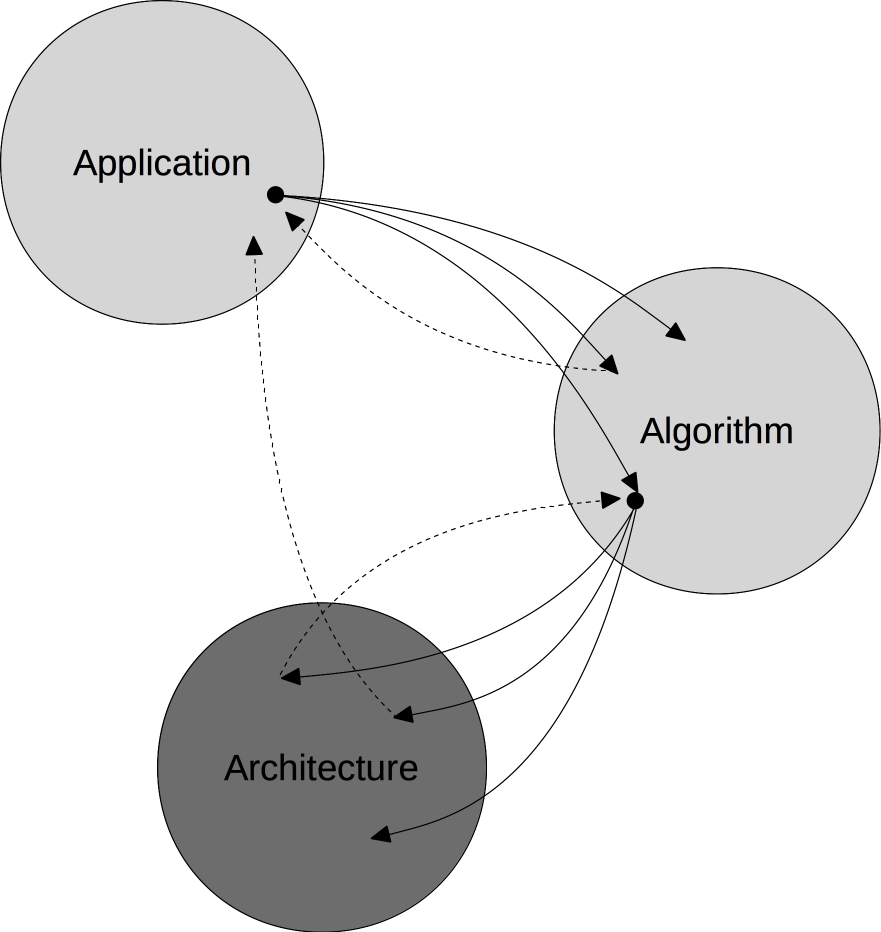
\includegraphics[scale=0.25]{figures/a3arch}
  \caption{A$^3$ model with the architecture domain marked}
  \label{fig:a3arch}
\end{figure}

A block diagram of the EEPSM algorithm is illustrated on figure \vref{fig:eepsmblock}. This block diagram is based on the pseudo code in section \vref{sec:eepsmpsuedocode}. The \textit{init. cost} block contains step 1 and 2 of the pseudo code, the $\mu$ block contains step 3 of the pseudo code, the \textit{horz. aggre} contains step 4 and 5, the \textit{vert. aggre.} block contains step 6 and 7 and the \textit{minimization} block will contain the minimization of the cost values to find the disparity values. This block diagram is created to divide the system into smaller subsystems. This is equal to go down an abstraction level i.e. synthesize in the Structure domain of the Y-Chart. This division into subsystems help limit size of systems which the different analyses and design processes is used on.\\
\begin{figure}[ht!]
  \centering
  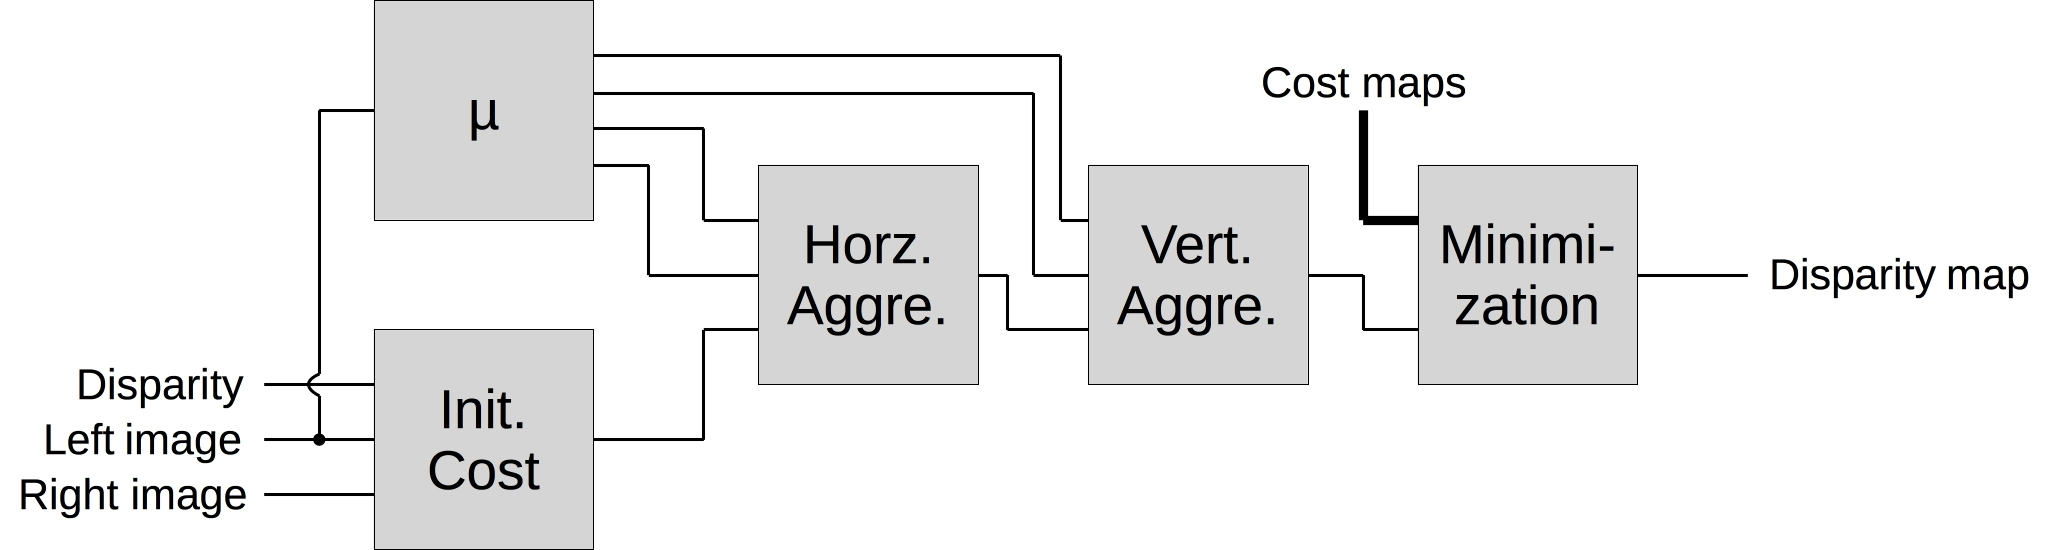
\includegraphics[width=0.75\textwidth]{figures/eepsmblockmain}
  \caption{Block diagram of the EEPSM algorithm}
  \label{fig:eepsmblock}
\end{figure}

To develop an FPGA hardware a finite state machine (FSM) and a data path are wanted. Before designing an FSM some processes and analyses should be performed. These processes are:
\begin{itemize}
\item Parallelism analysis
\item Allocation and scheduling
\item Assignment
\end{itemize}

Due to time constraint for the thesis, a final implementation was not achieved but the design process is shown at a lower abstraction level with the \textit{SAD cost} block which is a part of the \textit{init. cost} block in figure \vref{fig:eepsmblock}. 
\begin{figure}[ht]
  \centering
  \begin{subfigure}[t]{0.45\textwidth}
    \centering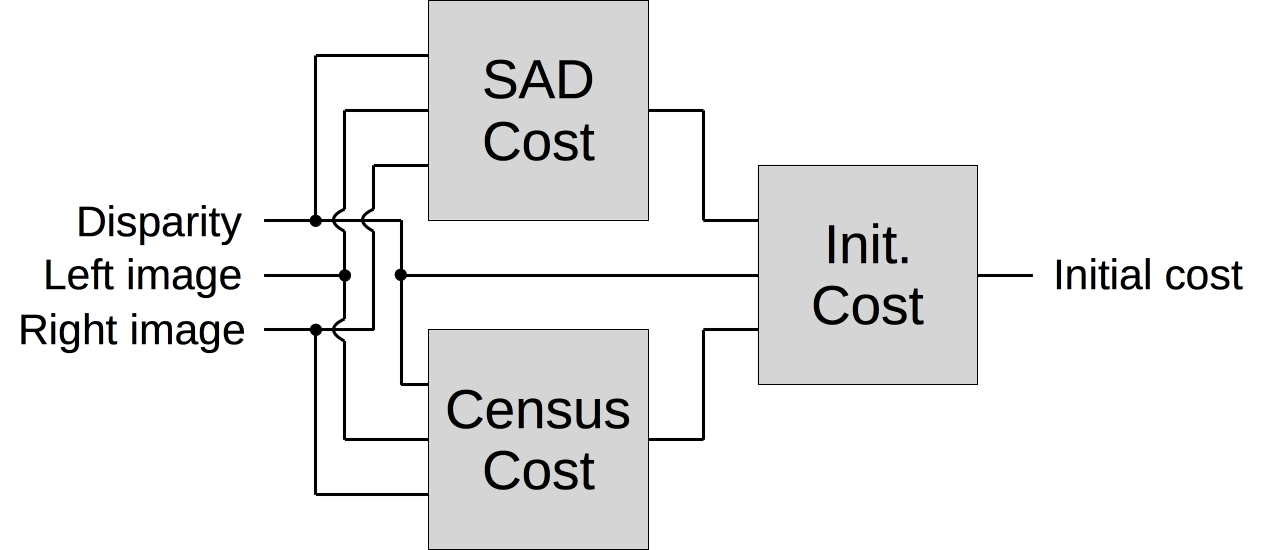
\includegraphics[scale=0.25]{figures/initcostblock.jpg}
    \caption{Init. Cost block diagram\label{fig:initcostblock}}
  \end{subfigure}\hspace{0.5cm}
  \begin{subfigure}[t]{0.45\textwidth}
    \centering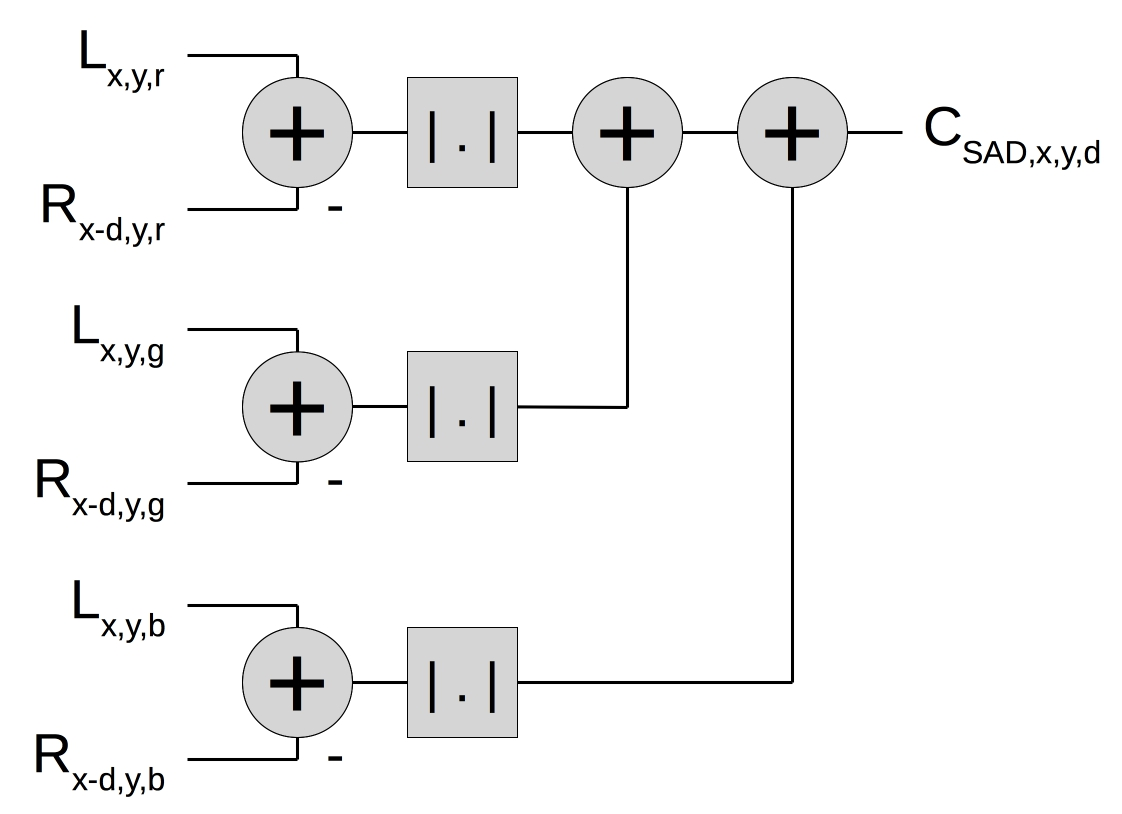
\includegraphics[scale=0.25]{figures/sadcostblock.jpg}
    \caption{Cost SAD block diagram\label{fig:sadcostblock}}
  \end{subfigure}
  \caption{Block diagrams\label{fig:initsadblock}}
\end{figure}

\section{Parallelism Analysis}\label{sec:paraanal}
The inherent parallelism of the system has been analyzed to find out which improvements can be made.\\

To find the parallelism in the system precedence graphs (PG) have to be created. With simple subsystems, the precedence graphs can be created  by looking at the system from end to start and for each operator find out which signal is needed and have to be calculated before.\\ 

\begin{figure}[ht!]
  \centering
  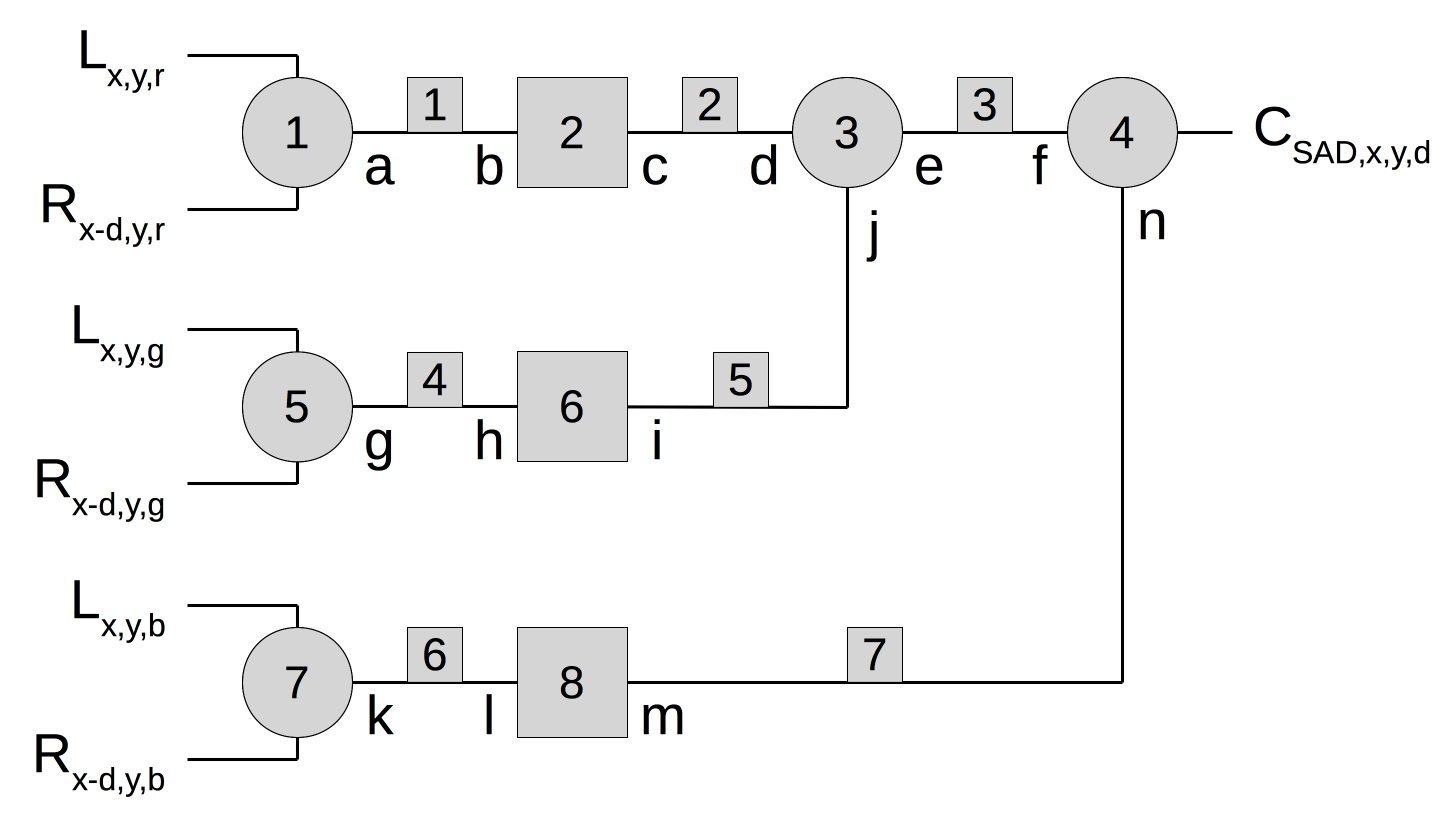
\includegraphics[scale=0.25]{figures/c_sad_sdfg.jpg}
  \caption{Synchronous data flow graph of the SAD cost block}
  \label{fig:c_sad_sdfg}
\end{figure}
Another method is to create a synchronous data flow graph (SDFG) and from the SDFG a matrix, $\uuline\Gamma$, can be created. This matrice expresses the relationship between the in- and outputs from each node in the SDFG and is called the \textit{topology} matrix. An example of an SDFG is illustrated on in figure \ref{fig:c_sad_sdfg}. In this example the topology matrix is then:
\begin{equation}
  \begin{array}{ c c c }
    & & \text{nodes} \\
  \uuline\Gamma = & \text{arcs} & 
  \begin{bmatrix}
   1 & -1 & 0 & 0 & 0 & 0 & 0 & 0 \\
   0 & 1 & -1 & 0 & 0 & 0 & 0 & 0 \\
   0 & 0 & 1 & -1 & 0 & 0 & 0 & 0 \\
   0 & 0 & 0 & 0 & 1 & -1 & 0 & 0 \\
   0 & 0 & -1 & 0 & 0 & 1 & 0 & 0 \\
   0 & 0 & 0 & 0 & 0 & 0 & 1 & -1 \\
   0 & 0 & 0 & -1& 0 & 0 & 0 & 1 \\
  \end{bmatrix}
  \end{array}
\end{equation}
If $rank(\uuline \Gamma) \leq s-1$ where $s$ is the number of nodes then a positive integer vector $\uline q$ can be found such that $\uuline\Gamma \cdot \uline q = \uline 0$. The resulting $\uline q$ is:
\begin{equation}
  \uline{q} =
  \begin{bmatrix}
  1 \\
  1 \\
  1 \\
  1 \\
  1 \\
  1 \\
  1 \\
  1
  \end{bmatrix}
\end{equation}
This $\uline q$ vector expresses how many times each node have to be executed within a period.\\

With $\uuline \Gamma$ and $\uline q$ a periodic admissible sequential sequence (PASS) can be found. This tells a sequential sequence in which the nodes can be executed and with it, a periodic admissible parallel sequence (PAPS) can be generated. To find the PASS generate a randomly ordered list of all the nodes, $L$. For each $\alpha \in L$ test if can be executed i.e. if data is available. If it can be executed then add it to the PASS, $\varphi$. This is repeated for each node and if every node have been scheduled in the PASS the number of times specified by $\uline q$ then continue to the next step.\\
For this example let $L=\{1, 2, 3, 4, 5, 6, 7, 8 \}$ then checking node 1 the data is available and is added to $\varphi$. After checking every node in $L$ once, $\varphi$ will be $\{1, 2, 5, 6, 7, 8 \}$. Since node 3 and 4 is missing in $\varphi$ then repeat the process. After this iteration $\varphi$ will be $\{1, 2, 5, 6, 7, 8, 3, 4 \}$. The PASS is only a sequential schedule but tells nothing about precedence relations and parallelism. For this, the precedence graph is used and it can be generated with the PASS found. Take one node at a time in the PASS and add it to the precedence graph and determine the precedence links. Figure \vref{fig:preceall} shows the progress towards a precedence graph.\\

\begin{figure}[ht]
  \centering
  \begin{subfigure}[t]{0.2\textwidth}
    \centering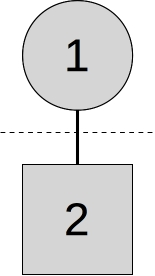
\includegraphics[scale=0.25]{figures/prece1.jpg}
    \caption{With only the 2 first nodes included \label{fig:prece1}}
  \end{subfigure}\hspace{0.5cm}
  \begin{subfigure}[t]{0.3\textwidth}
    \centering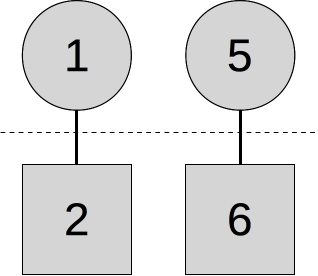
\includegraphics[scale=0.25]{figures/prece2}
    \caption{With only the 4 first nodes included\label{fig:prece2}}
  \end{subfigure}\hspace{0.5cm}
  \begin{subfigure}[t]{0.4\textwidth}
    \centering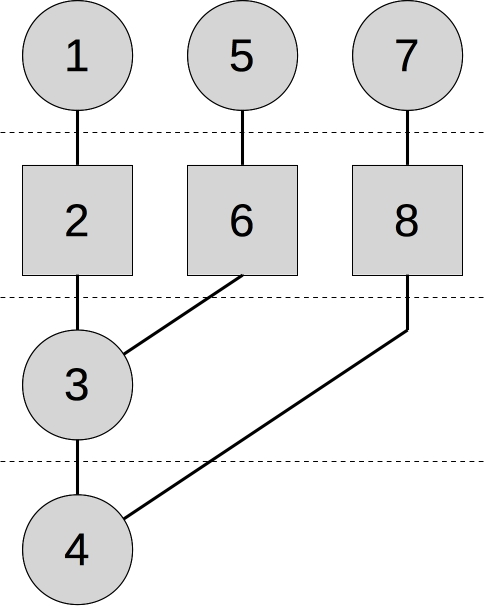
\includegraphics[scale=0.25]{figures/c_sadpre}
    \caption{With all the nodes in the SAD cost block\label{fig:prece3}}
  \end{subfigure}
  \caption{Precedence graph of the SAD cost block\label{fig:preceall}}
\end{figure}
The first figure shows the precedence graph when only the two first nodes from $\varphi$. When the next two nodes are added it is noticed how these are added next to node 1 and 2 since they have no precedence links to those nodes. The last figure shows the final precedence graph which can be used as a PAPS.\\

With the precedence graph found the next step towards a hardware design can be fulfilled. 

\section{Allocation and Scheduling}\label{sec:allocsched}
To develop a Finite State Machine (FSM) we need to know which hardware is allocated and when each operation is scheduled. This enables us to define some states for the FSM. From section~\ref{sec:paraanal} some a precedence graph are found and this graph shows how many FUs can run in parallel. \\

To create the FSM specification we need to introduce time into the precedence graphs to establish some states. To achieve this scheduling is used. There exist different methods for scheduling and some of these are:
\begin{itemize}
  \item Resource Constrained (RC)
  \item Time Constrained (TC)
\end{itemize}

\subsection{RC scheduling}
For both methods the first step is to create as soon as possible (ASAP) and as late as possible (ALAP) schedules. Then for the RC scheduling a ready list is created. This list contains a list of operations which are ready for scheduling and sorted by mobility. The mobility, $M(op)$, expresses the difference between the states in which the operation, $op$, have been scheduled in ASAP and ALAP schedules, e.i. $S_{ALAP}(op) - S_{ASAP}(op)$.\\

Figure \vref{fig:sch_asap_alap} shows an example of an ASAP and an ALAP schedule. As seen on the figure node 1-6 are part of the critical path and therefore mobility is 0 for each of these nodes. Nodes 7 and 8 both have a mobility of 1. \\
\begin{figure}[ht]
  \centering
  \begin{subfigure}[t]{0.45\textwidth}
    \centering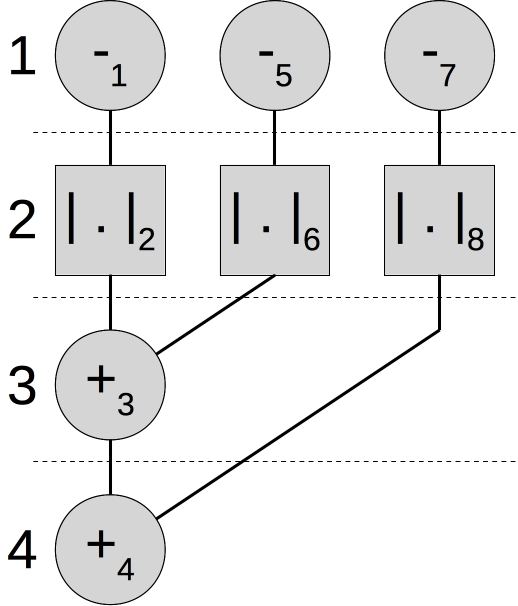
\includegraphics[scale=0.4]{figures/csadasap.jpg}
    \caption{Example of ASAP schedule\label{fig:sch_asap}}
  \end{subfigure}\hspace{0.5cm}
  \begin{subfigure}[t]{0.45\textwidth}
    \centering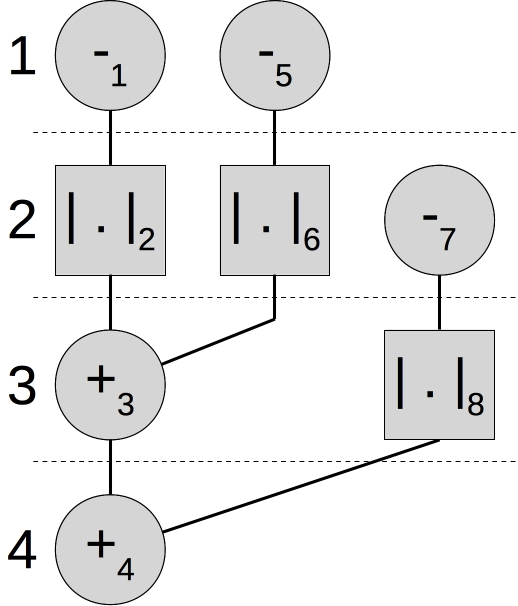
\includegraphics[scale=0.4]{figures/csadalap.jpg}
    \caption{Example of ALAP schedule\label{fig:sch_alap}}
  \end{subfigure}
  \caption{Illustration of ASAP and ALAP schedules for SAD cost block \label{fig:sch_asap_alap}}
\end{figure}

With mobility found for each node/operation then, a ready list can be generated. Add every ready node and then sort them by mobility. In the start the list would look like this: 1. node 1 ($M(-_1)=0$), 2. node 5 ($M(-_5)=0$) and 3. node 7 ($M(-_7)=1$).\\

If the system has 2 ALU available then node 1 and 5 can be scheduled to state 1 since they are higher on the ready list and there is no free ALU for the remaining node. The scheduled nodes are removed and the ready list is updated with newly available nodes. The list is still sorted by mobility and will now look like this: 1. node 2 ($M(|.|_2)=0$), 2. node 6 ($M(|.|_6)=0$) and 3. node 7 ($M(-_7)=1$). \\

Then nodes 2 and 6 are scheduled into state 2 since they have lower mobility than the rest of the ready list. The list is updated again and will look like this: 1. node 3 ($M(+_3)=0$) and 2. node 7 ($M(-_7)=1$).\\

Nodes 3 and 7 are scheduled into state 3 and the list is updated again: 1. node 8 ($M(|.|_8)=1$).\\

This is repeated until all nodes have been scheduled and the result is seen in figure \vref{fig:rc3alu}. This schedule uses 1 states more than the ASAP and ALAP but it reduces the cost since it uses 1 less ALU compared to the ALAP and ASAP schedules.\\

\begin{figure}[ht!]
  \centering
  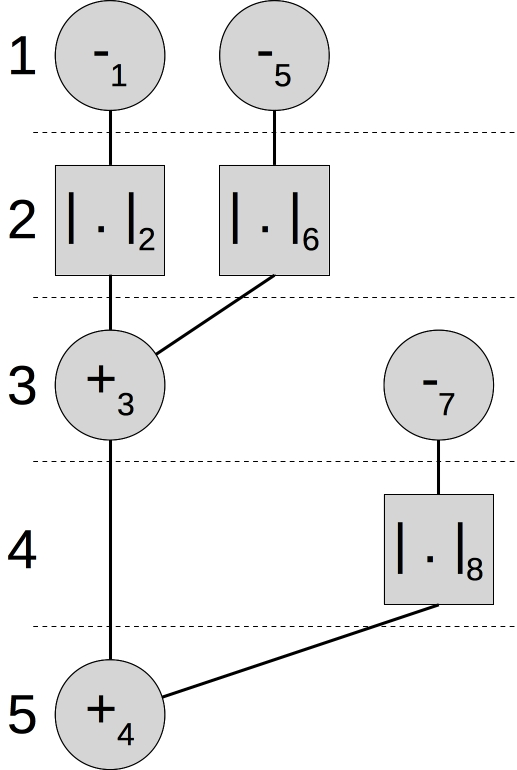
\includegraphics[scale=0.4]{figures/rccsad.jpg}
  \caption{RC schedule of the SAD cost}
  \label{fig:rc3alu}
\end{figure}
With this scheduling the allocation is performed before scheduling since the scheduling is constrained by how many FUs have been allocated.

\subsection{TC schedule}
The RC schedule improves the area cost of the architecture while the TC intends to improve the computational performance of the implementation. First, a maximum number of states is decided and then ASAP and ALAP schedules are generated and mobility ranges are found. Then some probabilities are assigned to each operation. These probabilities express the probability for the specified operation to be scheduled in each state in its mobility range e.g. node 7 in \ref{fig:sch_asap_alap} (p. \pageref{fig:sch_asap_alap}) have $1/2$ probability for being scheduled in each of state 1-2 if the maximum number of states is kept at 4. Figure \vref{fig:tc_prob} shows the probabilities for each node in figure \vref{fig:sch_asap_alap}.\\
\begin{figure}[ht!]
  \centering
  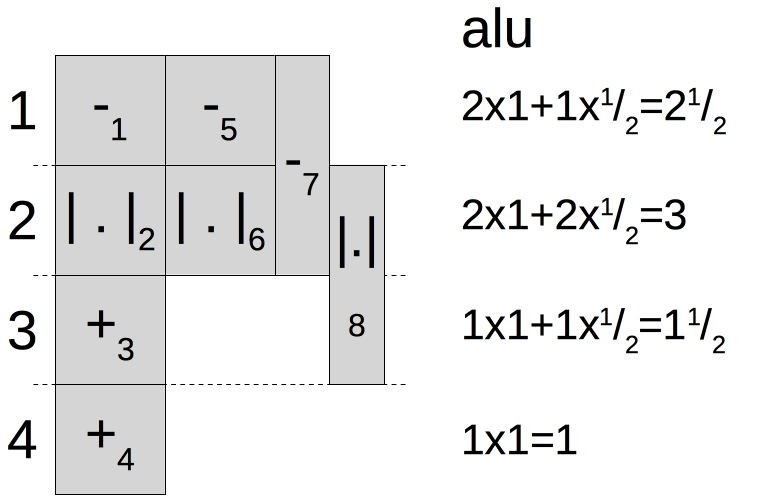
\includegraphics[scale=0.4]{figures/tccsadprop}
  \caption{Probabilities for each operation in figure \vref{fig:sch_asap_alap}}
  \label{fig:tc_prob}
\end{figure}

These probabilities can then be used to generate a force-directed schedule. With this scheduling the allocation of FUs is done after the schedule is found. 

\section{Assignment}
When a schedule have been found and some hardware have been allocated the hardware can be assigned. During the assignment process, the nodes are assigned to the allocated FUs. A lifetime analysis can also be performed the allocate register and assign the variables to these registers.\\
For the example, this step is skipped and it is chosen to directly implement an FSM from the ALAP schedule and let the Vivado software optimize the design. The resulting RTL architecture is shown on figure \vref{fig:csadrtl}. Due to time constraint the design process will stop at this point.
 
\begin{figure}[ht!]
  \centering
  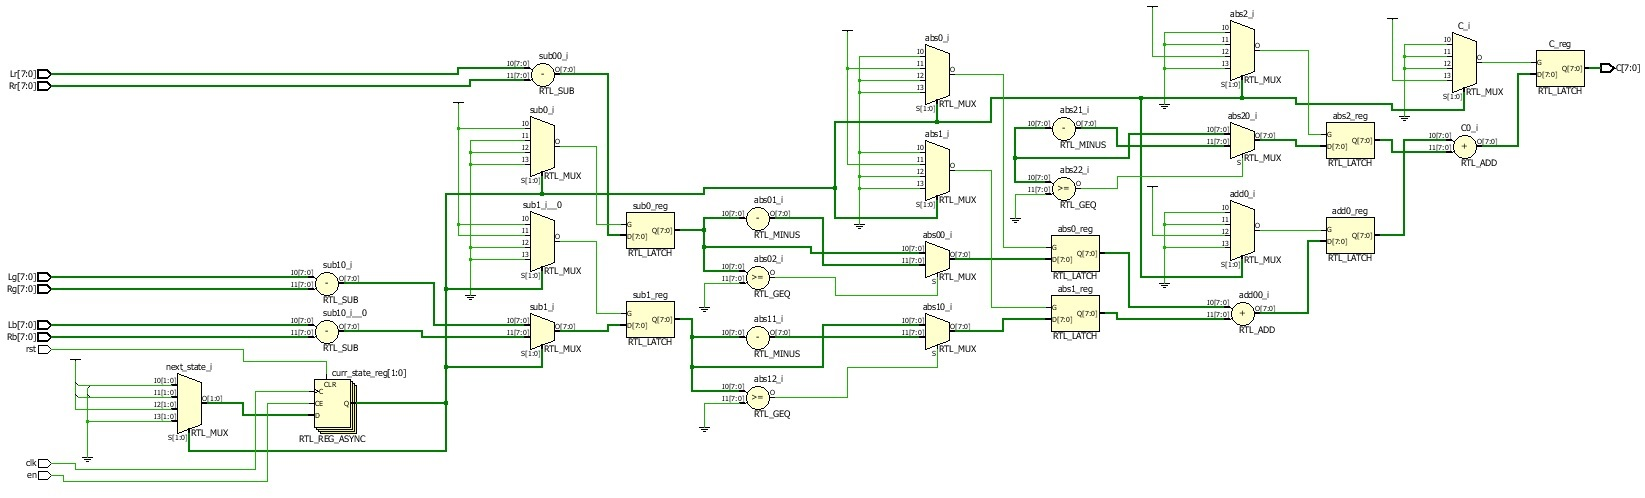
\includegraphics[width=0.95\textwidth]{figures/csad.jpg}
  \caption{SAD cost - RTL schematic}
  \label{fig:csadrtl}
\end{figure}

\section{Implementation challenges}
Some challenges were noticed at the higher abstraction levels and these will be described in this section.
 
\subsection{Exponential function} \label{sec:expfunc}
The exponential function is a high computational complex function which can be hard to implement. VHDL does not have an easy function to implement it and Xilinx Vivado does not have an IP core block with an exponential function. So another way to implement this function has to be found. \\

The exponential function can be defined by a power series:
\begin{flalign}
  && e^x &= \sum^{\infty}_{n=0} \frac{x^n}{n!} = 1 + x + \frac{x^2}{2!} + \frac{x^3}{3!} + \cdots && \label{eq:expseries}
\end{flalign} 
An approximation of the exponential function can be found by using a finite number of terms from power series definition. More terms results in a better approximation. \\

The input values for the exponential function will be in the range of $\left[ - \frac{255}{\sigma}; \frac{0}{\sigma} \right]$ where $\sigma$ through experiments have been chosen to be $38.1$ so the values will be in the interval $\left[ - 6.69; 0 \right]$. \\
\begin{figure}[ht!]
  \centering
  \begin{subfigure}[t]{0.50\textwidth}
    \centering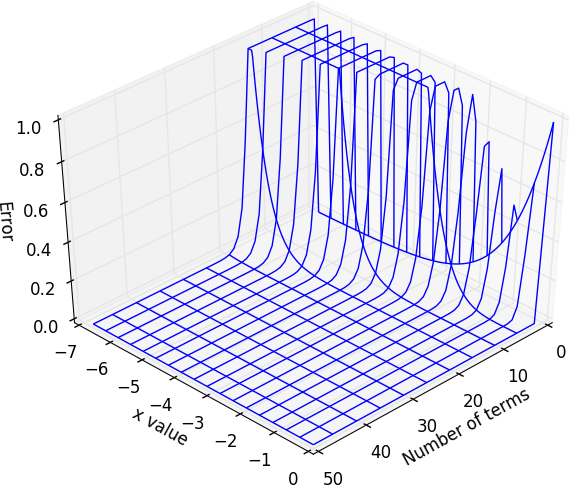
\includegraphics[width=\textwidth]{figures/exp_err_surf.png}
  \end{subfigure}\hspace{0.5cm}
  \begin{subfigure}[t]{0.40\textwidth}
    \centering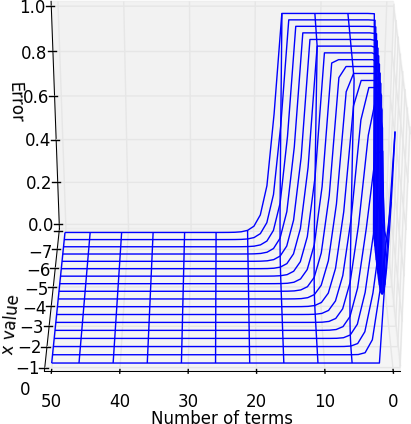
\includegraphics[height=6.5cm]{figures/exp_err_wire.png}
  \end{subfigure}
  \caption{Approximation error with respect to x value and number of terms seen from two views. Error values have been limited to the range $[0;1]$\label{fig:exp_err}}
\end{figure}

Figure \vref{fig:exp_err} shows the absolute error between the correct exponential value and the approximation with respect to the x value and number of terms used. It is noticed that a higher absolute value of x requires a higher amount of terms i.e. an x value of -1 requires at least 7 terms to have an error $\leq0.001$ while an x value of -6 requires at least 21 terms to achieve same precision.\\
\begin{figure}[ht!]
  \centering
  \begin{subfigure}[t]{0.50\textwidth}
    \centering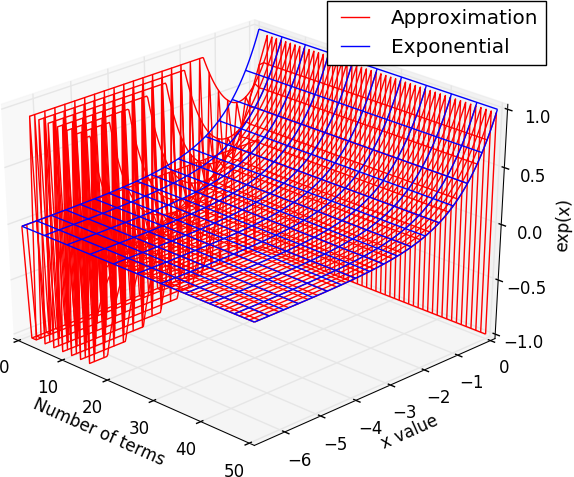
\includegraphics[width=\textwidth]{figures/exp_val_wire_1.png}
  \end{subfigure}\hspace{0.5cm}
  \begin{subfigure}[t]{0.40\textwidth}
    \centering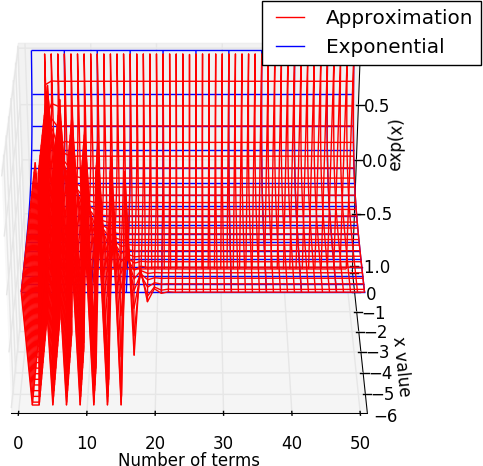
\includegraphics[height=6.5cm]{figures/exp_val_wire_2.png}
  \end{subfigure}
  \caption{Exponential values for approximation and the correct value with respect to x value and number of terms seen from two views. The values have been limited to the range $[-1;1]$\label{fig:exp_vals}}
\end{figure}

Figure \vref{fig:exp_vals} shows the result from the approximation (red surface) and the correct exponential values (blue surface). From this, it is noticed that the approximation at a low number of terms starts alternating between high positive and negative numbers when increasing the number of terms. The alternating positive and negative are due to the definition of $x^n$ in equation \ref{eq:expseries} and x being negative, and the large difference between the approximation and the correct result at a low number of terms is due to $x^n$ in the same equation starts out larger than the $n!$ but $n!$ grows quicker than $x^n$ when increasing the number of terms used.\\

To ensure that the error is $\leq 0.001$ at an x value of -6.69 then 23 terms have to be used and then the error is 0.00029. This power series could be implemented in hardware as a series of multipliers and adders. The $\frac{\cdot}{n!}$ of equation \ref{eq:expseries} can be implemented as multiplication with $\frac{1}{n!}$. But this implementation introduces an issue. Looking at the last term where $n=23$ and using the x value -6.69 the term is: $(-6.69)^{23} \cdot \frac{1}{23!}$. This term alone will use 24 multipliers and the result from $(-6.69)^{23}$ requires 65 bits for representing the final result as an integer and $\frac{1}{23!}$ requires 75 bits for representing it as a fixed-point value. This seems unfeasible to implement in hardware so alternative implementations have to be found.\\

There exist different methods to implement an exponential function. It can be implemented using a CORDIC engine and there is an IP core block of CORDIC available through Vivado. A CORDIC engine can calculate hyperbolic and trigonometric functions using iterative operations working on one bit at a time. The exponential function can be expressed using hyperbolic functions:
\begin{flalign}
  && e^x &= \cosh x + \sinh &&
\end{flalign}
The strength of the CORDIC is that it requires a low amount of hardware since it is an iterative algorithm but looking at computation performance other methods are better \cite{sudha2012novel}. One method which is better is using a look-up table containing the results. A look-up table can have a better computational performance but can require a high amount of memory \cite{sudha2012novel}. The x value in $e^x$ depends on the difference in intensity between two pixels hence the x value can only be 256 different values. A ROM containing these values needs address width of 8 bits. The only variable number which the exponential function depends on is the difference between intensity of two pixels. This difference can be used as the address to the memory cell containing the exponential value corresponding to that value i.e. if the difference is 3 then the memory cell at address 3 should contain $\exp(-3/\sigma)$.
The exponential values can be calculated before and just be inserted into the look-up table. To ensure that the lowest result, which is $e^{-6.69} = 0.0012$, will not be 0 at least 11 bits are needed. A look-up table of that size seems feasible to implement in hardware and therefore this solution is chosen.\\

\begin{figure}[ht!]
  \centering
  \includegraphics[width=0.95\textwidth]{figures/expRom}
  \caption{Schematic of ROM containing look-up table containing exponential values}
  \label{fig:exprom}
\end{figure}

A ROM containing the exponential values have been described in VHDL and synthesized for the Zedboard platform using Xilinx Vivado. Figure \vref{fig:exprom} shows a schematic of the implementation and table \vref{tab:exputili} shows how much hardware the implementation utilizes. From this, it is seen that a feasible implementation can be given with a look-up table.

\begin{table}
  \centering
  \begin{tabular}{r | c c}
   \toprule
   logic element & Utilization [$\cdot$] & Utilization [\%] \\
   \midrule
   LUT &  32 & 0.06 \\
   FF & 11 & 0.01 \\
   \bottomrule
  \end{tabular}
  \caption{Hardware utilization for ROM containing exponential values}
  \label{tab:exputili}
\end{table}

\subsection{Memory Issue in the EEPSM algorithm}
The EEPSM algorithm has a challenge with large images and disparity ranges such as those in this project in that it requires a large amount of memory for containing the cost of each pixel at each disparity value. Considering all the variables in the pseudocode in section \vref{sec:eepsmpsuedocode} and a variable size of 1 byte, keeping all these variables in memory will require \SI{13.8}{\giga\byte}. \\
\begin{table}[ht!]
  \centering
  \begin{tabular}{r | c | c | c | c | c | c | c |}
    Algorithm steps & 1 & 2 & 3 & 4 & 5 & 6 & 7 \\
    \hline
    Right image & \cellcolor{gray} &  \cellcolor{gray} &  \cellcolor{gray} & & & & \\
    Left image & \cellcolor{gray} &  \cellcolor{gray} &  \cellcolor{gray} & & & & \\
    SAD cost & \cellcolor{gray} & \cellcolor{gray} & & & & &  \\
    Cen. cost & \cellcolor{gray} & \cellcolor{gray} & & & & &  \\
    Combined cost & & \cellcolor{gray} & \cellcolor{gray} & \cellcolor{gray} & & & \\
    Permeability weights & & & \cellcolor{gray} & \cellcolor{gray} & \cellcolor{gray} & \cellcolor{gray} & \\
    Left aggregation & & & & \cellcolor{gray} & \cellcolor{gray} & & \\
    Right aggregation & & & & \cellcolor{gray} & \cellcolor{gray} & & \\
    Horizontal aggregation & & & & & \cellcolor{gray} & \cellcolor{gray} & \\
    Top aggregation & & & & & & \cellcolor{gray} & \cellcolor{gray} \\
    Bottom aggregation & & & & & & \cellcolor{gray} & \cellcolor{gray} \\
    Vertical aggregation & & & & & & & \cellcolor{gray} 
  \end{tabular}
  \caption{Lifetime for variables in the EEPSM algorithm \label{tab:memuse}}
\end{table}

Table \vref{tab:memuse} shows the lifetime of variables in the EEPSM algorithm. The algorithm steps in the table correspond to the steps in the pseudocode. From this, it can be seen that a maximum of 5 variables is needed to be kept in memory at the same time. This is at step 2 and this step requires \SI{4.6}{\giga\byte}. It is not feasible to implement with this memory requirement since the Zedboard only has \SI{512}{\mega\byte} DDR3 memory and 256 Quad-SPI Flash memory. The algorithm has to be changed to require less memory. Referring to the A$3$ model with this new knowledge the design process will go back to the algorithm domain and modify the algorithm to reduce memory usage. Referring to the Y-chart the design process will perform some iterations in the same abstraction level in the behavioral domain. Two methods to decrease the memory usage have been considered. \\

\begin{figure}[!ht]
  \centering
  \begin{subfigure}[t]{0.9\textwidth}
    \centering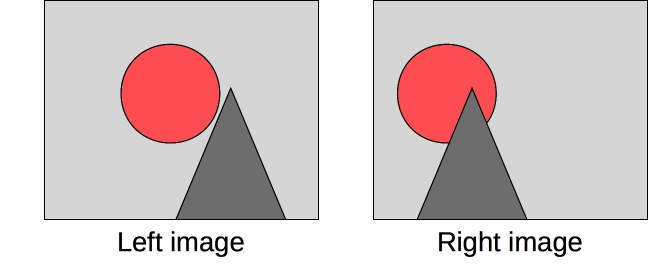
\includegraphics[scale=0.45]{figures/imgdiv1}
    \caption{Full images\label{fig:imgdiv1}}
  \end{subfigure}\\
  \begin{subfigure}[t]{0.9\textwidth}
    \centering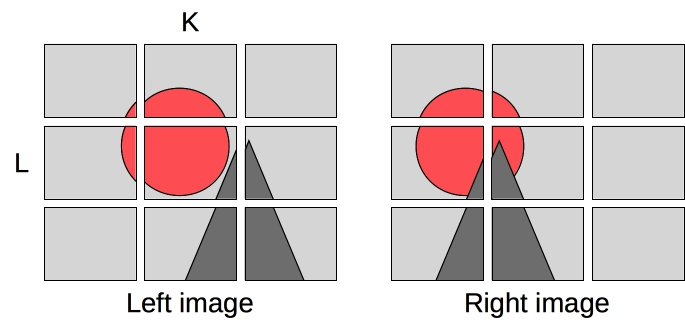
\includegraphics[scale=0.45]{figures/imgdiv2}
    \caption{Dividing the images along both y and x axes\label{fig:imgdiv2}}
  \end{subfigure}\\ \vspace{0.5cm}
  \begin{subfigure}[t]{0.9\textwidth}
    \centering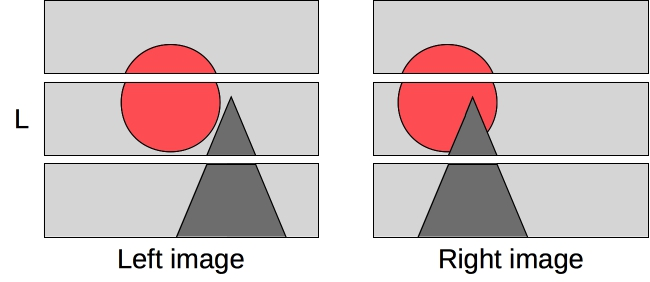
\includegraphics[scale=0.45]{figures/imgdiv3}
    \caption{Dividing the images along the y axis\label{fig:imgdiv3}}
  \end{subfigure}
  \caption{Illustration of dividing the images into smaller sub images\label{fig:imgdiv}}
\end{figure}

The first method suggests cutting the input images into smaller sub-images. This is illustrated on figure \vref{fig:imgdiv}. Figure \vref{fig:imgdiv2} shows an example where the images are divided along each axis and results in $K \times L$ sub-images. Performing the algorithm on one sub-image at a time reduces the memory usage by a factor proportional to $K \times L$ so in the case of $K = L = 3$ the memory usage could be reduced to \SI{515}{\mega\byte}. But some problems can occur when dividing this way. Looking at the triangle object in figure \vref{fig:imgdiv2} it is seen that the top of the triangle in the left image is in the rightmost column of sub-images while it is in the middle column of sub-images in the right image. This will result in a false matching when processing the sub-image containing the triangle top. To solve this issue the original image can instead be divided along the y-axis as illustrated on figure \vref{fig:imgdiv3}. Since the stereo matching only occurs along the x-axis, this way of dividing the image will not affect the matching the same way. The triangle top is, as seen in the figure, in the same sub-image. But it will require smaller rows to acquire the same reduction in memory as if dividing on both axes, since the reduction factor is proportional to $L$. Using the example in figure \vref{fig:imgdiv3}, where $L=3$, the memory will only be reduced to \SI{1.5}{\giga\byte} so $L$ have to be higher. It should be noted that with this method the stereo matching near borders between sub-images will be a bit worse than if working on full images since the aggregation will not include the cost values across the border. \\

\begin{figure}[ht]
  \centering
  \begin{subfigure}[t]{0.45\textwidth}
    \centering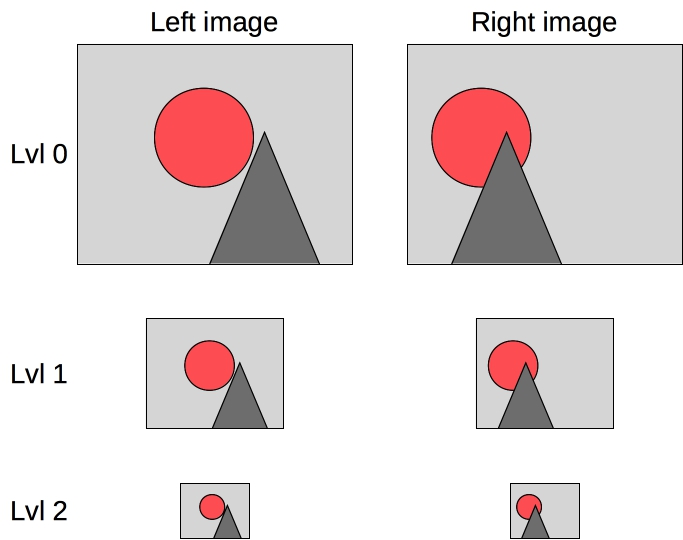
\includegraphics[width=\textwidth]{figures/imgdown1.jpg}
    \caption{Along both axes \label{fig:imgdown1}}
  \end{subfigure}\hspace{0.5cm}
  \begin{subfigure}[t]{0.45\textwidth}
    \centering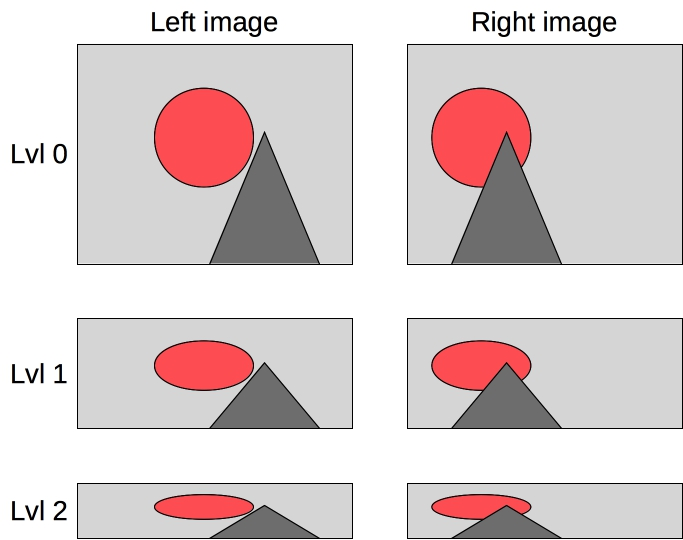
\includegraphics[width=\textwidth]{figures/imgdown2}
    \caption{Along y-axis\label{fig:imgdown2}}
  \end{subfigure}
  \caption{Image pyramid downsampling \label{fig:imgdown}}
\end{figure}

The second method to reduce memory use is using an image pyramid. An image pyramid is a down- and upsampling method which is often used in the computer vision field. It works by convolving the image with a gaussian kernel and then remove the even rows and columns which provide an image with a size reduced by a factor 4. This process can be repeated to downsample further. Each downsampled image is called a level in the pyramid where level 0 is the original size of the image, level 1 is the image downsampled once, etc. The original image size is reduced by a factor $2^{level+1}$ at each level. Figure \vref{fig:imgdown1} illustrates an image pyramid with 2 levels. A strength of this method is that beside memory usage reduction, fewer pixels are processed and this will result in the algorithm being faster. Using the figure as an example the memory usage at level 2 is reduced to \SI{579.4}{\mega\byte}.\\

Since pixels are removed then data is lost and the disparity precision will be lower than with the original images. The most important data are those along the x-axis since the stereo matching occurs along this axis. To avoid losing this data the image pyramid could be modified to only downsample along the y-axis. This is illustrated on figure \vref{fig:imgdown2}. With this modified image pyramid the size of the original image is reduced by a factor $2^{level}$ at each level. Using the example on figure \vref{fig:imgdown2} at level 2 the memory usage is reduced to \SI{1.16}{\giga\byte}. 
This method introduces some pre- and post-processing. The images have to be upsampled again after the algorithm has processed the image. The standard method for upsampling using an image pyramid is to double the size of the current image by inserting rows and columns of 0 next to each pixel or in the case of the modified version only rows will be inserted. Then the image is filtered with a gaussian kernel. An issue with this method is that since the upsampling is performed on the disparity map the calculated disparity values can be changed by the filtering. This is unwanted and instead of filtering the image, it has chosen to interpolate the rows containing 0 using linear interpolation.\\

\subsection*{Comparison of methods}
First, it is calculated how much the images should be divided or downsampled to reduce the memory usage below \SI{512}{\mega\byte} and then the python simulation created in section \ref{sec:simucomp} have been modified to use one of the two methods. The changes in stereo matching and runtime are presented in table \ref{tab:memmethodtable} and figure \ref{fig:memmetall} shows the resulting disparity maps.\\
For memory usage of method 1 to go below the available memory on the Zedboard, it has to be divided into at least 10 sub-images and the memory usage will then be \SI{463.5}{\mega\byte}. It should be noted that the image division results in the lower and upper border of each sub-image the disparity is equal to 0. This is resolved by setting the lower border equal to the row just above it and the upper border equal to the row just below it. This equal to a nearest neighbor interpolation.\\
For method 2 to go below the available memory it have to be downsampled 4 times and then the memory usage is equal to \SI{289.7}{\mega\byte}.\\

\begin{table}[!ht]
  \centering
  \begin{tabular}{c c c c c}
    \textbf{Method} &\textbf{ false matches [\%]} & \textbf{$\Delta$ false matches} & \textbf{runtime [s]} &  \textbf{$\Delta$ runtime [s]} \\
    None & 8.3 & - & 625 & - \\
    1 & 8.2 & -0.1 & 593 & -32  \\
    2 & 27.9 & +19.6 & 44 & -581 \\
  \end{tabular}
  \caption{Runtime og matching changes from each memory usage reduction method when using Motorcycle image set. \label{tab:memmethodtable}}
\end{table}

\begin{figure}[!ht]
  \centering
  \begin{subfigure}[t]{0.3\textwidth}
    \centering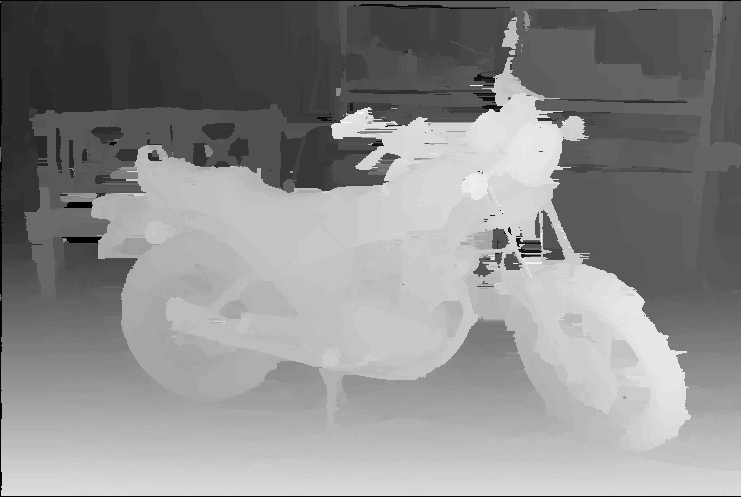
\includegraphics[width=\textwidth]{figures/mot_eepsm1}
    \caption{No method used \label{fig:memmetnone}}
  \end{subfigure}\hspace{0.5cm}
  \begin{subfigure}[t]{0.3\textwidth}
    \centering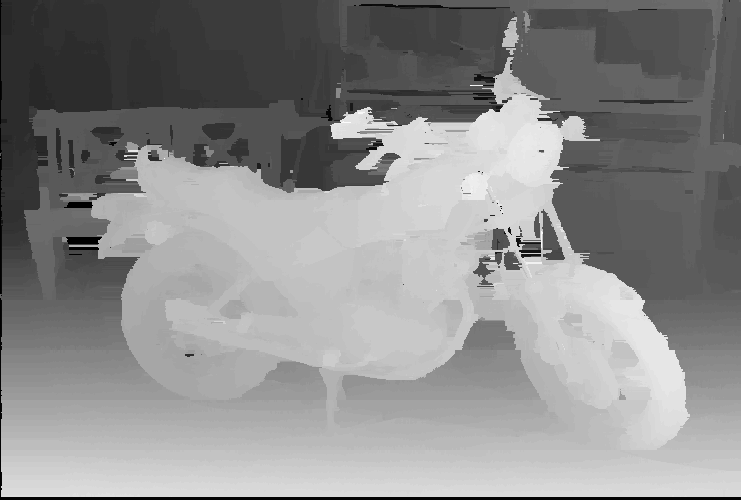
\includegraphics[width=\textwidth]{figures/mot_eepsm_div}
    \caption{Method 1 used\label{fig:memmetdiv}}
  \end{subfigure}\hspace{0.5cm}
  \begin{subfigure}[t]{0.3\textwidth}
    \centering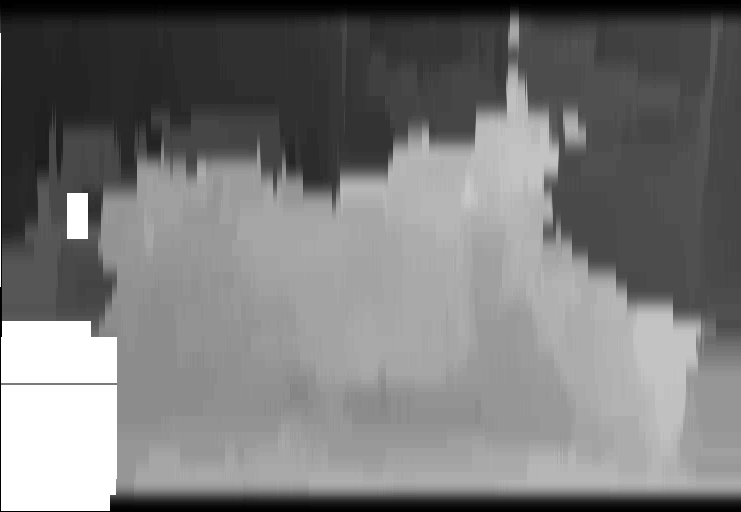
\includegraphics[width=\textwidth]{figures/mot_eepsm_down}
    \caption{Method 2 used\label{fig:memmetdown}}
  \end{subfigure}
  \caption{Resulting disparity maps using different memery usage reducing methods\label{fig:memmetall}}
\end{figure}

From the results, it can be seen that method 2 reduce the runtime by a large margin but the blurring in the image is too extensive and results in a lot of false matches. It also introduces some large blocks of errors seen in the lower left corner of the disparity map. Downsampling by only one level results in a fine disparity map with false matches equal to $9.5\%$ but already at level 2 the disparity map quality has degraded a lot and results in false matches to be $15.2\%$. Method 1 doesn't change neither the runtime or matching by much and therefore this method is chosen to reduce the memory usage. The decrease in false matches comes mainly from the top and bottom border of the disparity map since when using no method the algorithm doesn't change these borders and they are equal to zero whereas method 1 copies the line just above the bottom and below the top. If the same functionality is added to the original algorithm the false matches will be $7.9\%$. The reduction in run-time is believed by us to come from the python script processing smaller matrices. 

\section{Wrap-up}
A final FPGA implementation was not achieved due to time constraint for the thesis. But the basic process for design an FPGA hardware implementation is described. \\
Some challenges emerged during design at higher abstraction levels. One of these challenges were the implementation of exponential which was implemented using a lookup-table since the range of values were low. And another of these challenges is the memory usage due to large images and a high disparity range. The reduce the memory it were found that dividing the images into sub-images were feasible. 